\section{Análisis Experimental}

\begin{figure}
  \begin{center}
  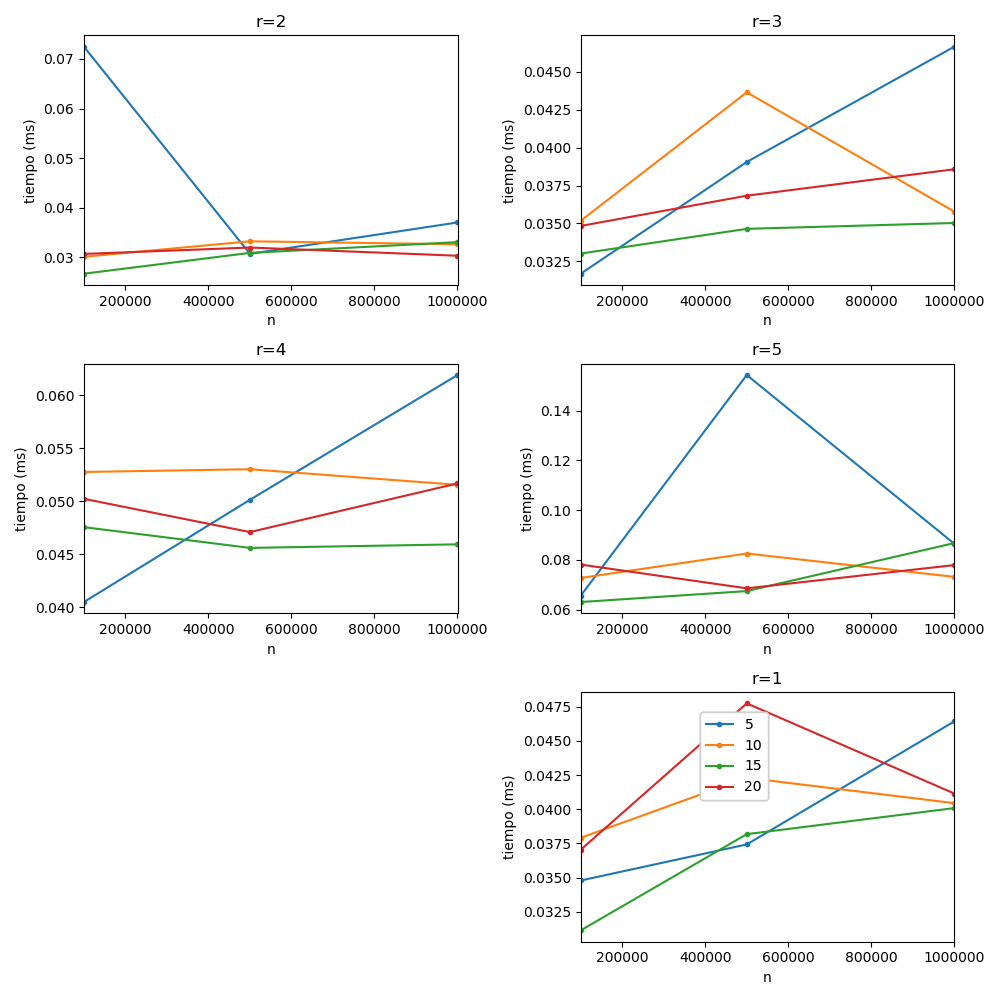
\includegraphics[width=.7\textwidth]{buscar_pos_n}
  \caption{Tiempo de búsqueda (positiva)
    según n, para distintos valores de r y k.}
  \label{fig:buscar-pos}
  \end{center}
\end{figure}


\begin{figure}
  \begin{center}
  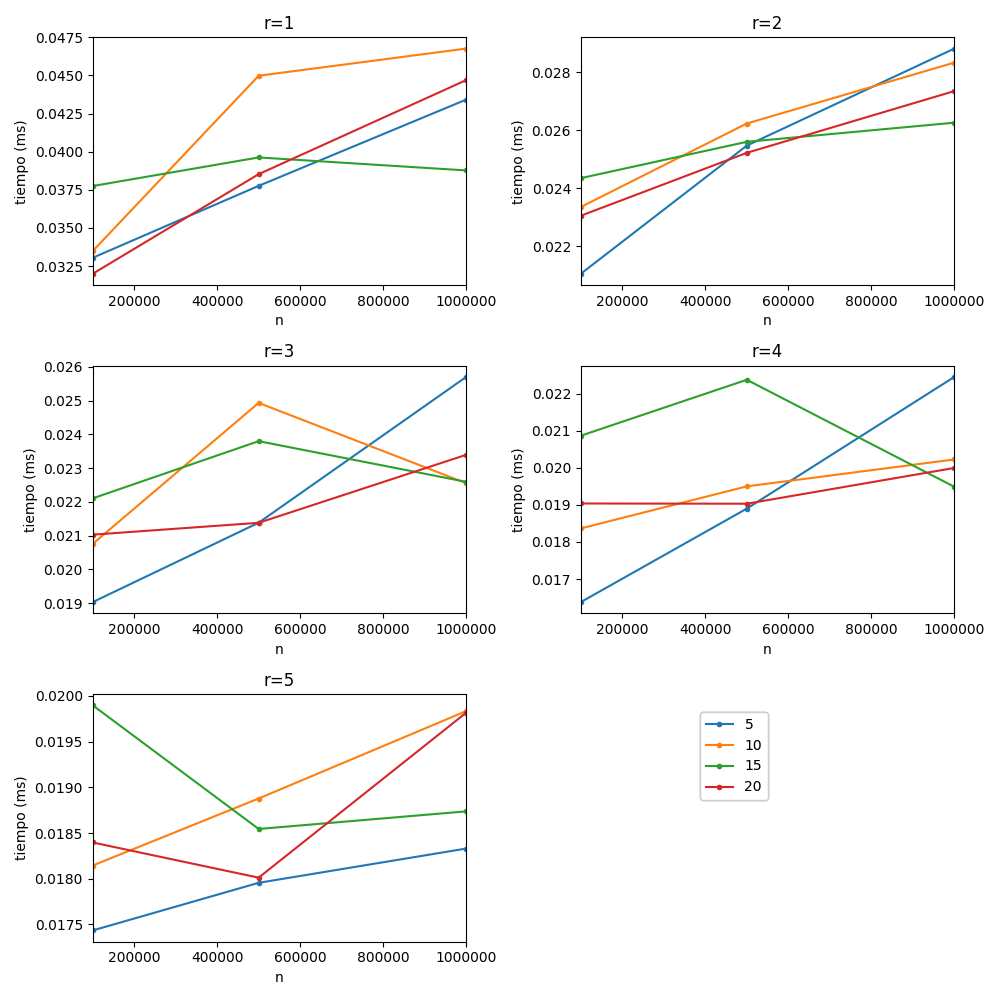
\includegraphics[width=.7\textwidth]{buscar_neg_n}
  \caption{Tiempo de búsqueda (negativa)
    según n, para distintos valores de r y k.}
  \label{fig:buscar-neg}
  \end{center}
\end{figure}

En las figuras \ref{fig:buscar-pos} y \ref{fig:buscar-neg} podemos
ver un crecimiento ligeramente cercano al logarítmico (que con tan solo 3
valores\footnote{Como se indica en la consigna} para \(n\) es dificil
distinguir).

La diferencia para distintos r (dado un k) se observa en la figura
\ref{fig:buscar}, y en todos los casos podemos observar que el árbol
con mayor r tiene un mejor rendimiento para las búsquedas tanto positivas como
negativas.

\begin{figure}
  \begin{center}
  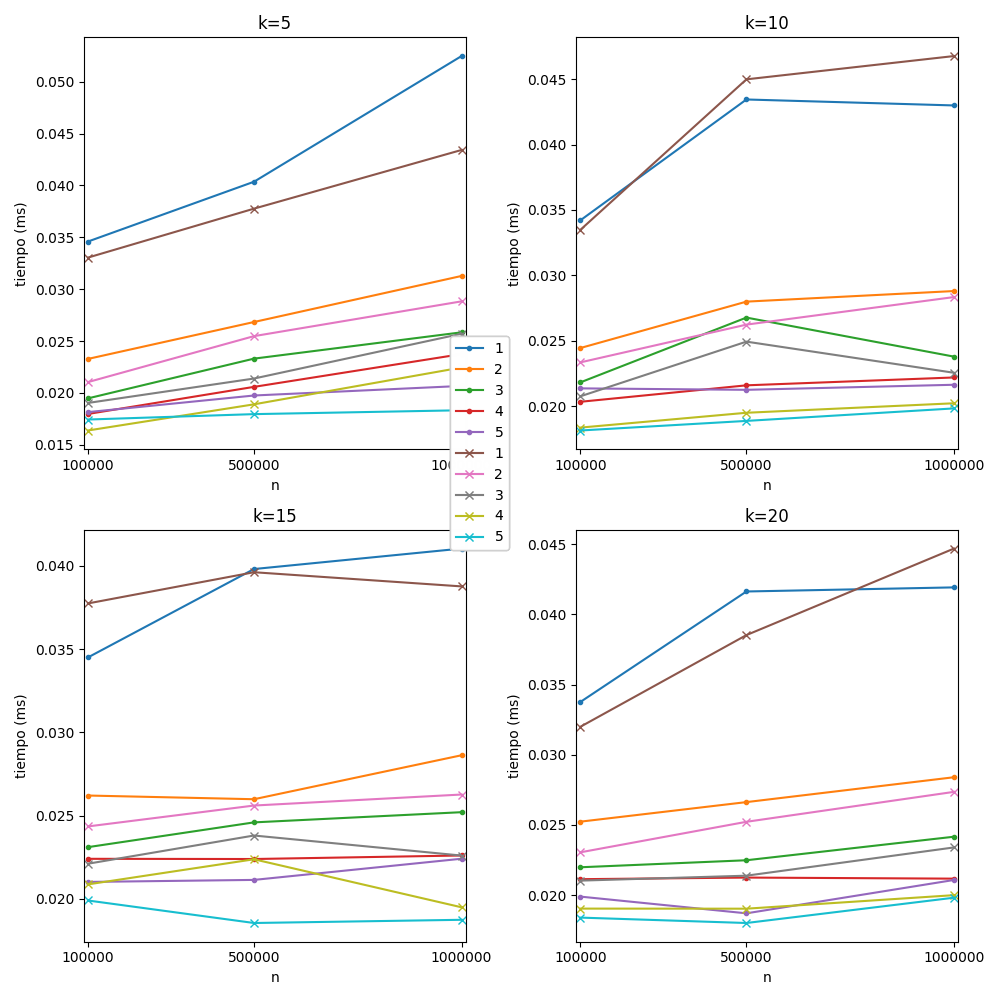
\includegraphics[width=.7\textwidth]{buscar_n}
  \caption{Tiempo de búsqueda (positiva y negativa)
    según n, para distintos valores de r y k.}
  \label{fig:buscar}
  \end{center}
\end{figure}

Esto se alinea con el desarrollo teórico, ya que \(r\) indica el factor de
ramificación, y cuanto mayor sea menos niveles debe recorrer hasta completar la
búsqueda.

Se observa una pequeña superioridad de las búsquedas negativas ante las positivas,
pero la diferencia no es significativa.

\begin{figure}
  \begin{center}
  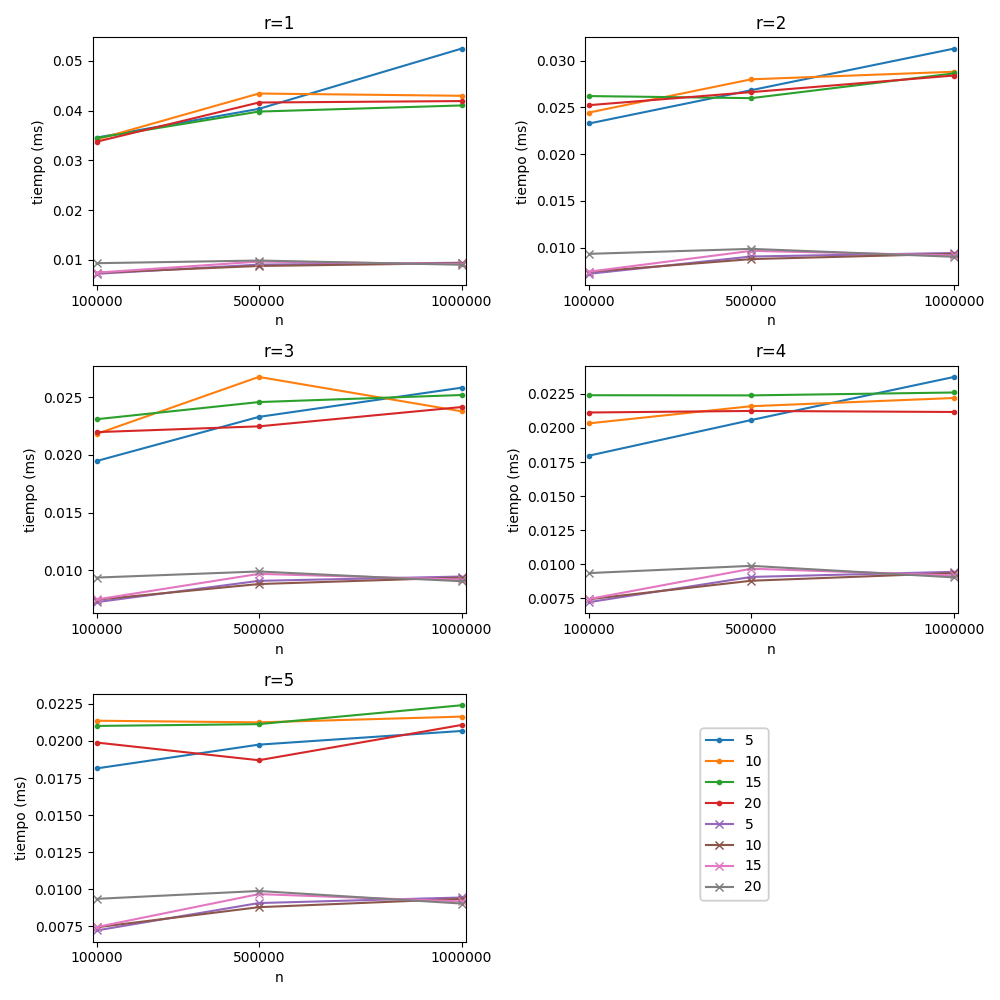
\includegraphics[width=.7\textwidth]{buscar_pos_kd_n}
  \caption{Tiempo de búsqueda (positiva)
    según n, para distintos valores de r y k, comparado con el arbol kd.}
  \label{fig:pos-kd}
  \end{center}
\end{figure}


\begin{figure}
  \begin{center}
  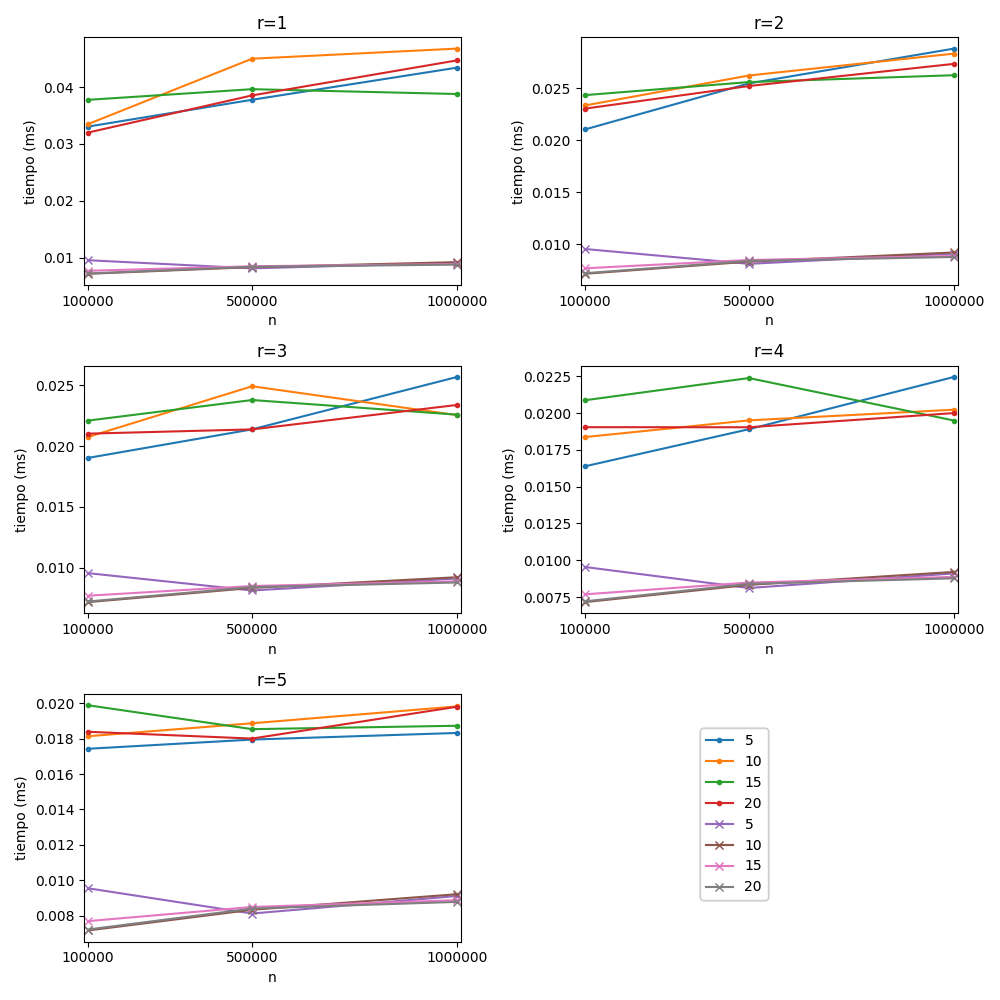
\includegraphics[width=.7\textwidth]{buscar_neg_kd_n}
  \caption{Tiempo de búsqueda (negativa)
    según n, para distintos valores de r y k, comparado con el arbol kd.}
  \label{fig:neg-kd}
  \end{center}
\end{figure}


En las figuras \ref{fig:pos-kd} y \ref{fig:neg-kd} podemos observar
una clara superioridad del árbol kd de búsqueda, logrando sus
búsquedas siempre por debajo de los 0.010ms, y esto se mantiene para
todo k y todo r. Ente los árboles kdr se observa variabilidad pero no
es signifiativa. Aún más, la creación de árboles
(fig. \ref{fig:armado}) muestra que la creación de arboles kd es
también superior, lo que es de esperar por la mayor complejidad del
algoritmos al tener que comparar r medianas.


\begin{figure}
  \begin{center}
  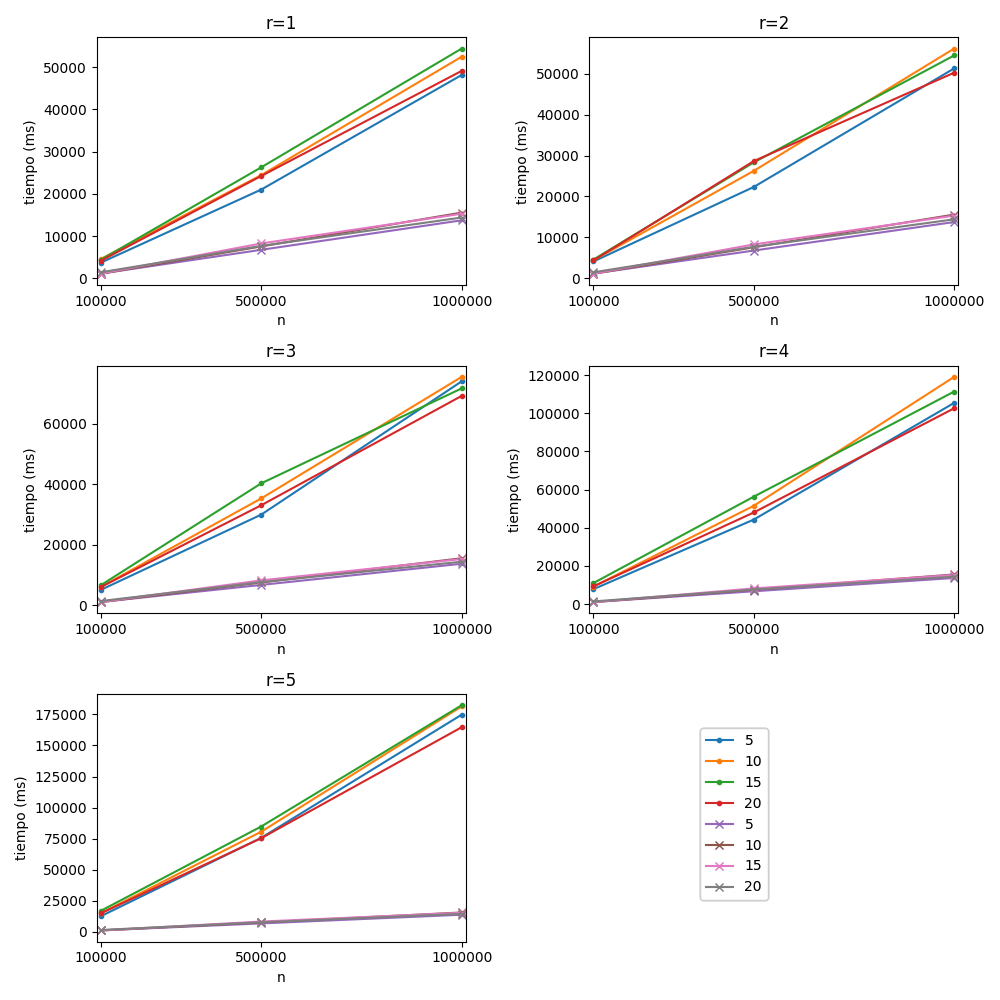
\includegraphics[width=.7\textwidth]{armado_n}
  \caption{Tiempo de creación de los arboles kd y kdr
    según n, para distintos valores de r y k.}
  \label{fig:armado}
  \end{center}
\end{figure}
